\chapter{Обзор литературы}
\section{Приложения квантовой информатики} \label{sec:ch1/sec1}

Метод квантового распределения ключа является одним из наиболее развитых на сегодняшний день практическим приложением квантовой информатики - области знаний на стыке фотоники, теории информации и квантовой физики, которая использует квантовые биты (кубиты), то есть квантовые системы, способные находиться в двух состояниях, для осуществления передачи, хранения и обработки информации [1]. Системы квантовой коммуникации позволяют их пользователям осуществлять рассылку симметричных криптографических ключей таким образом, что любые попытки вторжения нелегитимного пользователя в канал связи принципиально обнаруживаются. К другим перспективным приложениям квантовой информатики относятся квантовый компьютер - гипотетическое вычислительное устройство, работающее на принципах квантовой механики [2] и квантовая телепортация - передача квантового состояния на расстояние [3].


В последние годы отмечается рост интереса к прикладным аспектам квантовой информатики. В частности, основными фаворитами на получение Нобелевской премии 2012 года являлись работы по открытию и экспериментальному подтверждению квантовой телепортации под авторством основоположников квантовой криптографии Ч. Беннета и Ж. Брассара [4].  


Наибольшие прикладные успехи были достигнуты именно в системах квантовой коммуникации. В последние годы успехи в разработке экспериментальных образцов этих систем сопровождаются повышением интереса к их интегрированию в волоконно-оптические линии связи, что является необходимым условием для их широкого распространения этой технологии. В мире также появились первые коммерческие образцы [5], имеется большое количество патентов на разработки в данной сфере [6,7].


На сегодняшний день исследования в области квантовой рассылки ключа находятся в экспериментальной фазе: ранее были заложены основные принципы функционирования систем, предложен ряд способов генерации и обработки квантовых состояний, разработаны протоколы генерации ключа. Сегодня разработки ведутся с целью повышения технических характеристик систем: увеличения скорости и дальности распределения ключа, повышение спектральной эффективности, уменьшения воздействия шумов и факторов внешней среды, а также их интеграции в существующие линии связи телекоммуникационного стандарта. 

%%%%%%%%%%%%%%%%%%%%%%%%%%%%%%%%%%%%%%%%%%%%%%%%%%%%%%%%%%%%%%%%%%%%%%%%%%%%%%%%%%%%%%%%%%%%%%%%%%%%%%%%%%%%%%%%%%

\section{Системы квантовой коммуникации} \label{sec:ch1/sec2}

В современном мире требования к защите передаваемой  информации становятся все более жесткими в связи двумя проблемами:
\begin{enumerate}
	\item Условная стойкость математических алгоритмов шифрования.
Считается, что для взлома современных алгоритмов шифрования, злоумышленник не обладает достаточными вычислительными мощностями [8].
	\item Возможность появления квантового компьютера, обладающего необходимой вычислительной мощностью, чтобы в разумные сроки расшифровать закодированную информацию [9].
\end{enumerate} 


Наиболее выигрышную позицию в обозначенном выше вопросе занимает <<метод одноразового блокнота>>, предложенный Ж. Вернамом [10]. Идея этого метода заключается в обмене между легитимными пользователями секретными ключами, каждый из которых используется для шифрования только одного сообщения,  затем уничтожается. Для обеспечения безусловной стойкости применяют так называемый <<абсолютно стойкий ключ>> (АСК) [11], удовлетворяющий определенным требованиям:

\begin{enumerate}
	\item Ключ используется лишь один раз
	\item Длина ключа должна быть не менее длины шифруемого сообщения
	\item Ключ абсолютно случаен
	\item Ключ известен только легитимным пользователям
\end{enumerate}


В этих требованиях заложена проблема распространения АСК между доверенными лицами. И эту проблему можно решить, полагаясь на фундаментальные законы физики.


Итак, квантовая рассылка ключа (КРК) - направление в квантовой информатике, решающее проблему распределения <<абсолютно стойкого ключа>> между двумя и более легитимными пользователями [12].


Уникальность этого направления заключается в том, что секретность достигается за счет фундаментальных законов квантовой механики [12, 13]. Не существует способов измерения, усиления, копирования или разделения одних параметров системы без изменения других [14]. Таким образом, на основе анализа статистики принятых отсчётов можно утверждать об отсутствии или наличии в канале связи подслушивания, неизбежно влияющего на всю систему.


Принципиальная схема системы квантовой рассылки ключа (рис.\ref{fig:Fig_1}) включает в себя передатчик, именуемый Бобом (Bob), приёмник, именуемый Алисой (Alice), два связывающих их канала: квантовый и открытый. Также традиционно имеется нелегитимный пользователь (подслушиватель) - Ева (Eve) [12].


Принципиальная схема представлена на рис. \ref{fig:Fig_1}
 \begin{figure}[ht]
  \centering
  \includegraphics {Basic_scheme.pdf}
  \caption{\todo{Принципиальная схема системы квантовой рассылки ключа [12]}}
  \label{fig:Fig_1}
\end{figure}


По квантовому каналу, в качестве которого используется оптоволокно, происходит распределение ключа с использованием одиночных фотонов. Открытый же канал является незащищённым и используется для выяснения легитимными пользователями изменений статистики отсчетов и коррекции ошибок в первичном ключе, переданном по квантовому каналу связи [13].

%%%%%%%%%%%%%%%%%%%%%%%%%%%%%%%%%%%%%%%%%%%%%%%%%%%%%%%%%%%%%%%%%%%%%%%%%%%%%%%%%%%%%%%%%%%%%%%%%%%%%%%%%%%%%%%%%%

\section{Протоколы квантовой коммуникации} \label{sec:ch1/sec3}

Протоколом называется алгоритм формирование квантовых кодирующих последовательностей, то есть скоррелированных наборов бит у блоков отправителя и получателя с применением квантов света. "Классическими"  считаются протоколы BB84 и B92, разработанные основоположниками направления квантовой рассылки ключа. В основе первого лежит кодирование информации о ключе в 4 состояния, в качестве которых используются, например, поляризационные степени свободы, по два в каждом из двух базисов - вертикально-горизонтальном и диагональном [12]. Второго - кодирование в 2 состояния, \VCc{CHECK} ортогональных друг другу, в качестве которых традиционно используется фазы сигналов. Один из методов формирования кубитов - фазовое кодирование с использованием интерферометра Маха-Цендера [13]. Данный протокол реализуется следующим образом: на первом шаге Алиса случайным образом модулирует фазу светового импульса, выбирая сдвиг фазы, равный 0 или $\pi$. (При этом Алиса и Боб заранее договариваются, какие значения фазы будут соответствовать 0 и 1 в формируемой последовательности.) Боб независимо от Алисы случайным образом модулирует фазу идентичного светового импульса, выбирая сдвиг фазы, равный 0 или π и детектирует результат интерференции этих импульсов. Если интерференция конструктивна, то Боб верно угадал фазу (в нашем рассмотрении мы не учитываем влияние шумов), и полученный бит интерпретируется как 0 или 1 в зависимости от начальной договоренности. Если интерференция деструктивна (и анализатор Боба не детектирует импульс), то возможно два случая: или Боб неверно угадал фазу, заданную Алисой, или в этот временной отсчет не было послано ни одного фотона. Процесс повторяется снова для каждого импульса. По завершению передачи Боб сообщает Алисе, в какие промежутки времени он детектировал фотоны, не сообщая, какую модуляцию он использовал. Состояния, в которых Боб не детектировал импульсы, отбрасываются.


\begin{table} [htbp]
	\centering
	\caption{Пример формирования ключа по протоколу B92.}
	\label{tab:protocol}
	\begin{tabular}{| c | c | c | c | c |}
	 \hline	Алиса                              & \multicolumn{2}{|c|}{0}   & \multicolumn{2}{|c|}{1}   \\ \hline
	  Фаза Алисы					     	   & \multicolumn{2}{|c|}{0}   & \multicolumn{2}{|c|}{1}   \\ \hline
	  \makecell{Боб выбирает \\ фазу}	    	   & 0      	                   & 180    & 0 	& 180      \\ \hline
	  \makecell{Боб детектирует \\ фотон}      & ДА                        & НЕТ    & НЕТ   & ДА       \\ \hline
	  \makecell{Алиса и Боб \\ разделяют бит}  & ДА                        & НЕТ    & НЕТ   & ДА       \\ \hline
	\end{tabular}%
\end{table}


Простейшая схема B92 (модификация интерферометра Маха-Цендера, каждое из плеч которого находится у одного из участников) представлена на рисунке \ref{fig:Fig_2}.
 

 \begin{figure}[ht]
  \centering
  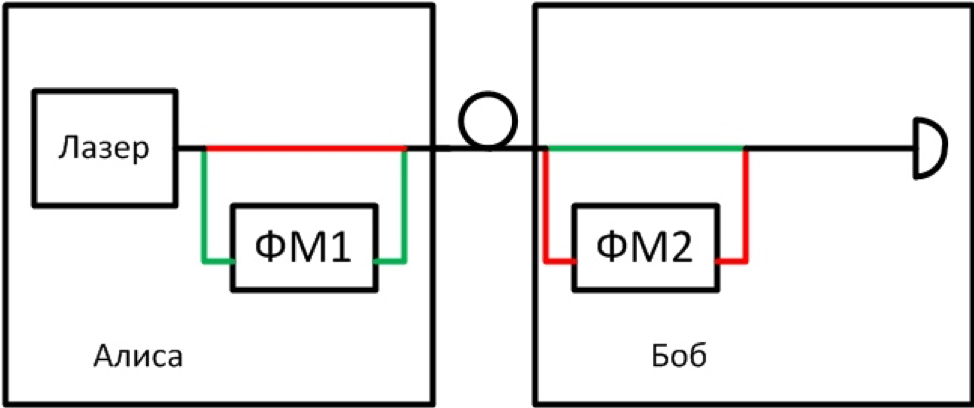
\includegraphics {Fig_2.png}
  \caption{\todo{Принципиальная схема системы квантовой коммуникации с фазовым кодированием [13]}}
  \label{fig:Fig_2}
\end{figure}

Испущенный лазером импульс разделяется Алисой на две части: одна идет по "короткому" пути (красный1) и проходит через модулятор фазы (ФМ1), а второй по "длинному" пути (зеленый1). Информация кодируется изменением фазы в ФM1. После прохождения по линиям связи, импульсы приходят в такой же интерферометр на стороне Боба, где снова разделяются, формируя три вида импульсов. Первый, прошедший дважды по "короткому" пути (зеленый 2) и последний, дважды прошедший по "длинному" (красный 2), не несут никакой информации. Средний является результатом интерференции импульсов, прошедших пути красный1-красный2 и зеленый1-зеленый2. Чтобы детектировать полученный в результате интерференции импульс необходимо его отделить от мощного импульса красный1-зеленый2 с помощью электро-оптического затвора ЭЗ и направить на детектор одиночных фотонов ДОФ. Импульс красный1-зеленый2 впоследствии может использоваться в качестве опорного импульса, то есть сигнализировать о факте прибытия квантового импульса.

%%%%%%%%%%%%%%%%%%%%%%%%%%%%%%%%%%%%%%%%%%%%%%%%%%%%%%%%%%%%%%%%%%%%%%%%%%%%%%%%%%%%%%%%%%%%%%%%%%%%%%%%%%%%%%%%%%

\section{Системы квантовой коммуникации на боковых частотах модулированного излучения} \label{sec:ch1/sec4}

Метод квантового распределения ключа на боковых (поднесущих) частотах модулированного излучения (КРКПЧ) был предложен в работе [16] и развивался в работах [17, 18]. Основными особенностями являются: простота по сравнению с указанными выше аналогами благодаря исключению влияния поляризации, а также отказу от работы по принципу интерферометра Маха-Цендера ввиду необходимости постоянного проведения достаточно сложной юстировки; высокая скорость передачи информации; возможность мультиплексирования сигнала с разделением по длине волны.

 
Генерация криптографического ключа по протоколу B92 в данной системе происходит следующим образом [19]:


 Световой пучок генерируется источником монохроматического излучения, в данном случае лазерным диодом. Излучение подвергается амплитудной или фазовой модуляции с помощью модулятора Алисы (ФМ1). В простейшем случае применяется периодическая синусоидальная модуляция. В результате модуляции в спектре сигнала появляются две боковые частоты, отстоящие от основной частоты оптического сигнала на величину частоты модулирующего радиочастотного сигнала. Для передачи квантового сигнала используются боковые частоты при выполнении условия $\mu \ll 1$ ( $\mu$ - среднее число фотонов в импульсе). Далее световой пучок ослабляется с помощью аттенюатора до уровня энергии одиночных фотонов. Мощность излучения на боковых частотах должна быть значительно ниже, чем на центральной частоте. Для того, чтобы среднее время между двумя генерируемыми фотонами не превышало один такт кодирования, регулируется индекс модуляции, зависящий от амплитуды модулирующего сигнала.  Ослабленный сигнал на центральной частоте представляет собой опорный световой пучок. Кодирование происходит благодаря внесению в модулирующий сигнал некоторого фазового сдвига. Блок отправителя соединен с блоком получателя волоконно-оптической линией связи. При достижении приёмного устройства сигнал подвергается повторной модуляции по аналогии с устройством отправителя (ФМ2). При этом в модулирующий сигнал также вносится случайный фазовый сдвиг. Мощность излучения на боковых частотах зависит от значений фазового сдвига, внесенных на передающем устройстве и приемном устройстве. Если они совпали, т.\:е. разность фаз двух модулирующих радиочастотных сигналов равна нулю ($\phi$A-$\phi$В=$0$), на боковых частотах наблюдается конструктивная интерференция, и мощность оптического сигнала отлична от нуля. В случае, когда модулирующие радиочастотные сигналы Алисы и Боба находятся в противофазе, т.\:е. разность фаз модулирующих сигналов равна $\pi$ ($\phi$A-$\phi$В=$\pi$), наблюдается деструктивная интерференция, и мощность сигнала на боковых частотах равняется нулю [16].
 
 
При конструктивной интерференции значениям выбранных сдвигов фаз (0 или π) соответствуют, по договоренности, биты (0 или 1). Боб по открытому каналу сообщает Алисе моменты времени, когда совпали их сдвиги фаз, и та, в свою очередь, отбрасывает лишнюю информацию. Так генерируется <<просеянный>> ключ, который подлежит процедуре коррекции ошибок. 

 \begin{figure}[ht]
  \centering
  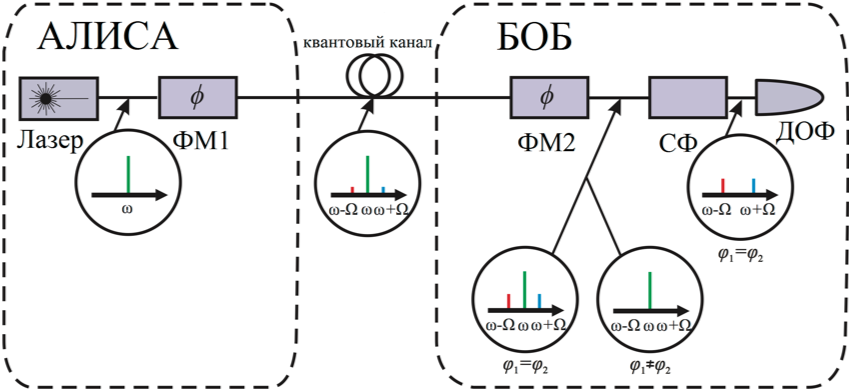
\includegraphics {Fig_3.png}
  \caption{\todo{Принципиальная схема системы квантовой коммуникации на боковых частотах модулированного излучения}}
  \label{fig:Fig_3}
\end{figure}


%%%%%%%%%%%%%%%%%%%%%%%%%%%%%%%%%%%%%%%%%%%%%%%%%%%%%%%%%%%%%%%%%%%%%%%%%%%%%%%%%%%%%%%%%%%%%%%%%%%%%%%%%%%%%%%%%%

\section{Измерительное оборудование в системах квантовой коммуникации} \label{sec:ch1/sec5}


Системы квантовой коммуникации (СКК) оперируют с крайне низкоинтенсивным излучением в волоконно-оптических линиях связи (ВОЛС), где в среднем в каждом тактовом отсчете сосредоточена энергия менее одного фотона. Детекторы одиночных фотонов (ДОФ) способны улавливать подобные сигналы, что делает их неотъемлемой частью СКК. Условно ДОФ можно разделить на две группы: широкодоступные и узкоспециализированные. Очевидно, что детекторы из второй группы, например, криогенные термоэлектрические детекторы (QVD) [17] и детекторы, основанные на поглощении в холодном атомном паре [18], не могут быть использованы серийно в производстве систем СКК. Поэтому в данном разделе рассматриваются основные виды которые широко применимых ДОФ:

\begin{enumerate}
	\item на основе лавинных фотодиодов для однофотонного излучения (single-photon avalanche diode, SPAD);
	\item использующие полевой транзистор, обогащенный квантовыми точками, с оптическим затвором (quantum-dot optically gated field-effect transistor, QDOGFET);
	\item использующие сверхпроводящие нанопроволоку (superconducting nanowire single-photon detector, SNSPD);
	\item использующий джозефсоновский переход (superconducting-tunnel-junction detector, STJ);
	\item использующие сенсор, реагирующий на переход материала из сверхпроводящего состояния в проводящее (transition-edge sensor, TES);
	\item счетчик фотонов видимого света (visible-light photon counter, VLPC) и твердотельный фотоумножитель (solid-state photomultiplier, SSPM).
\end{enumerate}

На основании сравнительной характеристики будет оценена целесообразность использования данных ДОФ для СКК.

\subsection{Лавинные фотодиоды для однофотонного излучения}

ДОФ этого типа используют процесс, схожий с тем, что происходит в фотоумножителе [19]. В отличие от фотоумножителя, в фотодиоде поглощение фотона рождает электрон-дырочную пару, которая порождает аналогичное увеличение числа заряженных частиц благодаря напряжению, приложенному вдоль кристаллической решетки полупроводника. Лавинные фотодиоды, используемые для ИК излучения, имеют низкие типичные показатели квантовой эффективности 10-20~\%  (доля излучения, которая успешно переведена в электрический сигнал и зарегистрирована). Они также характеризуются достаточно высокими значениями частоты темновых срабатываний (ложные срабатывания детектора в отсутствие входящего излучения, зачастую вызванного теплом окружающей среды), поэтому диод охлаждают до 210-250 К, например, термоэлектрическими охладителями. Даже в этом случае уровень темновых отсчётов для коммерческих ДОФ данного типа составляет порядка 1-10 кГц. Для лавинных детекторов характерна остаточная пульсация, когда электроны из лавины ненадолго <<застревают>>, например, в дефектах и, освобождаясь, порождают вторичные лавины. Необходимо некоторое время для выхода в штатный режим работы, поэтому у таких диодов обычно относительно высокое мертвое время (время, когда детектор сразу после срабатывания не может повторно зарегистрировать сигнал), что может ограничить тактовую частоту следования квантовых сигналов в СКК.

\subsection{ДОФ, использующий полевой транзистор, обогащенный квантовыми точками, с оптическим затвором}

Совмещение полевого транзистора с оптическим затвором из квантовых точек, расположенных между стоком и истоком, позволяют добиться регистрации одиночных ИК фотонов [20]. Квантовые точки захватывают заряженные частицы, рожденные падающим светом, изменяя приложенное электрическое поле, что ведет к изменению протекающего по транзистору тока - по данному изменение и производится детектирование сигнала. Однако низкое быстродействие данного детектора не соответствует типовым системам СКК. Квантовая эффективность не превышает 15~\%, а максимальная тактовая частота следования квантовых сигналов составляет всего 50 кГц. Кроме того, для работы данного ДОФ необходимы низкие рабочие температуры (от 70 К и ниже). При этом вероятность темновых срабатываний относительно высока.

\subsection{ДОФ, использующие сверхпроводящую нанопроволоку}

Данный тип ДОФ является одним из самых быстрых. Он способен регистрировать квантовые состояния с частотой следования до единиц гигагерц [21]. Основным элементом здесь служит площадка со сверхпроводящей тонкой проволокой (superconducting nanowire), запитанная током немного меньшим, чем критический, выше которого волокно выходит из сверхпроводящего режима. В таком случае поглощенный фотон оставляет небольшой участок нагретым и, соответственно, в проводящем состоянии. Поэтому ток начинает огибать этот участок с нормальной проводимостью. В результате ток превышает критическое значение, что приводит к переходу в проводящий режим всего участка вдоль ширины волокна. Появление участка с сопротивлением выражается в соответствующем скачке напряжения во внешней цепи, что и свидетельствует о детектировании фотона. Поскольку данный механизм детектирования требует очень узкой проволоки (порядка 100 нм), его складывают меандром, для создания эффективной рабочей поверхности. Для повешения эффективности детектирования, сверху волокно покрывают отражающей поверхностью, что в итоге образует резонатор, значительно улучшающий характеристики детектора. В подобных устройствах используют в основном проволоку из нитрида ниобия, однако из-за высокого коэффициента отражения у данного материала - необходимо просветляющее покрытие, благодаря которому можно добиться высокого значения квантовой эффективности до 60~\%. Ввиду того, что детектор работает в сверхпроводящем режиме, ему необходимы низкие рабочие температуры менее 4 К. В этом режиме он характеризуется низким уровнем темновых отсчётов ($10^{-2}$-$10^2$ Гц), что важно при реализации дальнодействующих СКК.

\subsection{ДОФ, использующие джозефсоновский переход}

Основным элементов для данного типа детекторов служит джозефсоновский переход - две части сверхпроводника разделенных сверхтонким (порядка 1 нм) диэлектриком, см., например, [22]. Фотон, падающий на сверхпроводящую область, вызывает распад большого числа куперовских пар электронов (квазичастицы), т.\:к. его энергия в тысячи раз больше энергии связи. Свободные электроны после распада пар способны туннелировать через диэлектрик во вторую часть сверхпроводника с крайне высокой вероятностью. Поскольку рабочая температура детектора на порядок ниже переходной температуры в сверхпроводящее состояние, куперовских пар распавшихся за счет иных процессов, нежели за счет поглощенных сигнальных фотонов, значительно меньше, что позволяет однозначно зарегистрировать однофотонное излучение. Таким образом, данный вид детекторов позволяет детектировать фотоны с эффективностью, не превышающей 45~\%, частотой следования фотонов порядка десятков кГц, однако при крайне низких рабочих температурах 0,37 К.

\subsection{Детекторы одиночных фотонов, использующий сенсор, реагирующий на переход материала из сверхпроводящего состояния в проводящее}

Данный сенсор работает по принципу болометра: при поглощении излучения повышается температура сенсора [23]. Для достижения чувствительности к одиночным фотонам необходима крайне малая теплоемкость поглощающего материала, и температурный сенсор должен обладать чрезвычайно высоким откликом на малое изменение температуры. Это возможно при изготовлении сенсора из тонкого сверхпроводящего материала, и его работы точно при температуре перехода из сверхпроводящего режима в обычный (порядка 100 мК) так, что небольшое изменение температуры отражается в значительном изменении сопротивления. Большей точности измерения колебаний сопротивления можно добиться, используя сверхчувствительный магнитометр, основанный на сверхпроводящем квантовом интерферометре (SQUID). Данный вид детекторов обладает самым большим показателем квантовой эффективности среди прочих - 95~\% для фотонов в ИК области. Несмотря на это, максимальная частота следования фотонов ограничена порогом в 100 кГц.

\subsection{ДОФ видимого света и твердотельный фотоумножитель}

С точки зрения квантовой эффективности, данный детектор может сравниться с предыдущим, но в области видимого света, где она достигает 90~\% [24]. Принцип работы схож с лавинным диодом, но в данном случае не электрон, а дырка, выбитая падающим излучением, ускоряется к легированной части полупроводника, где уже рождает электронную лавину. Несмотря на высокое значение квантовой эффективности, остальные параметры достаточно низки: максимальная скорость детектирования фотонов составляет 100 кГц, частота темновых срабатываний велика - не менее 20 кГц. Схожими по конструкции и принципу работы являются твердотельные фотоумножители [25]. Они обладают широкой спектральной восприимчивостью, что, в свою очередь, требует экранирования от дальнего ИК излучения, которое не представляет интереса.

\subsection{Cравнительная характеристика ДОФ для СКК}

Ниже представлена таблица 1, в которой представлены ключевые параметры детекторов, описанных в предыдущих разделах.

\begin{table} [htbp]
	\centering
	\caption{Сравнительные характеристики распространённых ДОФ.}
	\label{tab:SPD_compare}
	\begin{tabular}{| c | c | c | c | c |}
	
	 \hline \makecell{Тип \\детектора} & \makecell{Рабочая T,\\~K} & \makecell{Квантовая \\эффективность,\\~\%} & \makecell{Максимальная \\частота \\регистрации \\квантовых \\сигналов} & \makecell{Темновые отсчеты, \% \\(от частоты \\регистрации \\квантовых \\сигналов)}   \\ \hline
	  SPAD         & 210-250    & < 20    & 300 МГц     & < 0,1   \\ \hline
	  STJ	   	   & < 1        & > 45    & 10 кГц  	& < 0,1      \\ \hline
	  QDOGFET      & < 80       & < 15    & 50 кГц      & < 1       \\ \hline
	  TES          & < 0,1      & > 90    & 1 МГц       & < 0,01       \\ \hline
	  \makecell{VLPC\\/SSPM} & < 10      & < 90    & 100 кГц       & < ~20      \\ \hline
	  SNSPD          & < 10      & < 60    & 3 ГГц       & < 0,0001       \\ \hline
	  
	\end{tabular}
\end{table}

На основе выполненного сравнения можно сделать следующие выводы. 


Лавинные фотодиоды для однофотонного излучения (SPAD) рекомендуется использовать для СКК. Это объясняется тем, что они работают при температурах, которые возможно обеспечить без дополнительного охлаждающего криогенного оборудования, имеют оптоволоконный интерфейс и обладают максимальной частота регистрации квантовых сигналов ниже, чем предполагаемая частота смены фазы квантовых состояний электроникой СКК. Относительно низкая квантовая эффективность и высокий уровень темновых срабатываний, однако, позволяет использовать данный вид детекторов на малых и средних дистанциях при небольших потерях в линиях ВОЛС (до 10-15 дБ).


ДОФ, использующий джозефсоновский переход (STJ) не рекомендуется использовать для приложений СКК ввиду низкой максимальной частоты регистрации квантовых сигналов и крайне низких рабочих температур, обеспечение которых является сложным технологическим процессом, увеличивающим их стоимость.


ДОФ, использующий полевой транзистор, обогащенный квантовыми точками, с оптическим затвором (QDOGFET) не рекомендуется использовать для приложений СКК по причине низкой скорости срабатывания.


ДОФ, использующий сенсор, реагирующий на переход материала из сверхпроводящего состояния в проводящее (TES) не рекомендуется использовать для приложений СКК ввиду низкой максимальной частоты регистрации квантовых сигналов и крайне низких рабочих температур, обеспечение которых является сложным технологическим процессом.


Счетчик фотонов видимого света (VLPC) и твердотельный фотоумножитель (SSPM) не рекомендуется использовать для приложений СКК по причине низкой скорости срабатывания.


ДОФ, использующий сверхпроводящую нанопроволоку (SNSPD) рекомендуется использовать для приложений СКК, т.\:к. они работают при температурах жидкого гелия, что возможно обеспечить в свою очередь и компенсируется высокими ключевыми показателями, которые обеспечат штатную работу системы СКК. Данный тип детекторов следует использовать в каналах с относительно высокими потерями (от 15 дБ). 

%%%%%%%%%%%%%%%%%%%%%%%%%%%%%%%%%%%%%%%%%%%%%%%%%%%%%%%%%%%%%%%%%%%%%%%%%%%%%%%%%%%%%%%%%%%%%%%%%%%%%%%%%%%%%%%%%

\section{Атаки злоумышленника Евы} \label{sec:ch1/sec6}

\todo{Написать про отличие моделей от практической реализации.Квантовый взлом \\ Атака с разделением пучка фотонов. \\Атака типа перехват. \\Атака типа перехват-пересылка. \\Атака на детектор на основе ЛФД. \\ Атака с навязыванием ключа ( Faked-state attack) \\ Атака на SNSPD }

\subsection{Атака с разделением пучка фотонов} 


\subsection{Атака типа перехват} 


\subsection{Атака типа перехват-пересылка} 


\subsection{Атака на детектор на основе ЛФД} 


\subsection{Атака с навязыванием ключа ( Faked-state attack)} 


\subsection{Атака на SNSPD} 


%%%%%%%%%%%%%%%%%%%%%%%%%%%%%%%%%%%%%%%%%%%%%%%%%%%%%%%%%%%%%%%%%%%%%%%%%%%%%%%%%%%%%%%%%%%%%%%%%%%%%%%%%%%%%%%%%%

\section{Известные контрмеры против атак на измерительное оборудование} \label{sec:ch1/sec7}

\todo{Предложены ряд решений. Практически апробированы не были.}

\subsection{Статистика счета фотонов}

\subsection{Измерение фототока}

\subsection{MDI-протокол}

\subsection{Twin-Field протокол}


%%%%%%%%%%%%%%%%%%%%%%%%%%%%%%%%%%%%%%%%%%%%%%%%%%%%%%%%%%%%%%%%%%%%%%%%%%%%%%%%%%%%%%%%%%%%%%%%%%%%%%%%%%%%%%%%%%

\section{Выбор направления исследований. Цели и задачи работы} \label{sec:ch1/sec8}

Системы квантовой коммуникации на боковых частотах модулированного излучения зарекомендовали себя, как перспективное направление коммерчески доступных устройств квантового распределения ключа с практически значимыми характеристиками мирового уровня, подтвержденными в ряде научных публикаций в международных изданиях, формализованным доказательством безусловной секретности используемого протокола \VCc{ТАК?}, применением на нескольких полигонах, развернутых на территории Российской Федерации, совместной с ведущими компаниями в области телекоммуникационной связи, банковского сектора и региональными инжиниринговыми центрами. 


С научной и инженерной точки зрения данный класс систем имеет большой задел:

\begin{enumerate}
	\item Экспериментальная демонстрация передачи квантовых состояний на основе технологии квантовой коммуникации на боковых частотах модулированного излучения в телекоммуникационной линии связи дальностью свыше 250 км. 
	\item Разработка функциональной схемы и экспериментальная реализация оптико-электронного устройства квантовой передачи информации на боковых частотах, включающую подсистему непрерывной синхронизации модулей отправителя и получателя, подсистему компенсации неконтролируемого изменения поляризации в оптическом волокне.
	\item Экспериментально продемонстрировано спектральное уплотнение каналов на боковых частотах. 
	\item Разработка функциональной схемы и экспериментальная реализация оптико-электронного устройства квантовой передачи информации на боковых частотах, включающую подсистему непрерывной синхронизации модулей отправителя и получателя, подсистему компенсации неконтролируемого изменения поляризации в оптическом волокне.
	\item Экспериментальная демонстрация применимости данной технологии для квантового распределения ключа в открытом пространстве, а не только в волоконно-оптических линиях связи. 
\end{enumerate}


Однако, устойчивость квантовых систем передачи информации на боковых частотах к воздействию нелегитимного пользователя на измерительной оборудование ранее не была исследована. 


{\aim} данной работы является исследование возможностей злоумышленника по получению секретного ключа с использованием атак на измерительное оборудование систем квантовой коммуникации на боковых частотах и разработка методов противодействия атакам.


Для~достижения поставленной цели необходимо было решить следующие {\tasks}:
\begin{enumerate}
  \item Исследование устойчивости детектора одиночных фотонов, применяемого в системах квантовой коммуникации на боковых частотах, к атакам с выведением из режима Гейгера (<<ослеплением>>). 

  \item Оценка возможностей злоумышленника при атаке с выведением из режима Гейгера для систем квантовой коммуникации на боковых частотах. 

  \item Разработка оптической схемы системы квантовой коммуникации, устойчивой к атакам на измерительное оборудование. 

  \item Разработка протокола квантовой рассылки ключа, устойчивого к атаке на измерительное оборудование. 

\end{enumerate}
%%%%%%%%%%%%%%%%%%%%%%%%%%%%%%%%%%%%%%%%%%%%%%%%%%%%%%%%%%%%%%%%%%%%%%%%%%%%%%%%%%%%%%%%%%%%%%%%%%%%%%%%%%%%%%%%%%
\chapter{Оформление различных элементов} \label{ch:ch1}

\section{Форматирование текста} \label{sec:ch1/sec1}

Мы можем сделать \textbf{жирный текст} и \textit{курсив}.

\section{Ссылки} \label{sec:ch1/sec2}
Сошлёмся на библиографию.
Одна ссылка: \cite[с.~54]{Sokolov}\cite[с.~36]{Gaidaenko}.
Две ссылки: \cite{Sokolov,Gaidaenko}.
Много ссылок: %\cite[с.~54]{Lermontov,Management,Borozda} % такой «фокус»
%вызывает biblatex warning относительно опции sortcites, потому что неясно, к
%какому источнику относится уточнение о страницах, а bibtex об этой проблеме
%даже не предупреждает
\cite{Lermontov, Management, Borozda, Marketing, Constitution, FamilyCode,
Gost.7.0.53, Razumovski, Lagkueva, Pokrovski, Methodology, Nasirova, Berestova,
Kriger}%
\ifnumequal{\value{bibliosel}}{0}{% Примеры для bibtex8
    \cite{Sirotko, Lukina, Encyclopedia}%
}{% Примеры для biblatex через движок biber
    \cite{Sirotko2, Lukina2, Encyclopedia2}%
}%
.
И~ещё немного ссылок:
\cite{Article,Book,Booklet,Conference,Inbook,Incollection,Manual,Mastersthesis,
Misc,Phdthesis,Proceedings,Techreport,Unpublished}
% Следует обратить внимание, что пробел после запятой внутри \cite{}
% обрабатывается ожидаемо, а пробел перед запятой, может вызывать проблемы при
% обработке ссылок.
\cite{medvedev2006jelektronnye, CEAT:CEAT581, doi:10.1080/01932691.2010.513279,
Gosele1999161,Li2007StressAnalysis, Shoji199895, test:eisner-sample,
test:eisner-sample-shorted, AB_patent_Pomerantz_1968, iofis_patent1960}
\ifnumequal{\value{bibliosel}}{0}{% Примеры для bibtex8
}{% Примеры для biblatex через движок biber
    \cite{patent2h, patent3h, patent2}%
}%
.

\ifnumequal{\value{bibliosel}}{0}{% Примеры для bibtex8
Попытка реализовать несколько ссылок на конкретные страницы
для \texttt{bibtex} реализации библиографии:
[\citenum{Sokolov}, с.~54; \citenum{Gaidaenko}, с.~36].
}{% Примеры для biblatex через движок biber
Несколько источников (мультицитата):
% Тут специально написано по-разному тире, для демонстрации, что
% применение специальных тире в настоящий момент в biblatex приводит к непоказу
% "с.".
\cites[vii--x, 5, 7]{Sokolov}[v"--~x, 25, 526]{Gaidaenko}[vii--x, 5, 7]{Techreport},
работает только в \texttt{biblatex} реализации библиографии.
}%

Ссылки на собственные работы:~\cite{vakbib1, confbib1}

Сошлёмся на приложения: Приложение \ref{app:A}, Приложение \ref{app:B2}.

Сошлёмся на формулу: формула \eqref{eq:equation1}.

Сошлёмся на изображение: рисунок \ref{fig:knuth}.

Стандартной практикой является добавление к ссылкам префикса, характеризующего тип элемента.
Это не является строгим требованием, но позволяет лучше ориентироваться в документах большого размера.
Например, для ссылок на рисунки используется префикс \textit{fig},
для ссылки на таблицу -- \textit{tab}.

В таблице \ref{tab:tab_pref} приложения \ref{app:B4} приведён список рекомендуемых
к использованию стандартных префиксов.

\section{Формулы} \label{sec:ch1/sec3}

Благодаря пакету \textit{icomma}, \LaTeX~одинаково хорошо воспринимает
в~качестве десятичного разделителя и запятую ($3,1415$), и точку ($3.1415$).

\subsection{Ненумерованные одиночные формулы} \label{subsec:ch1/sec3/sub1}

Вот так может выглядеть формула, которую необходимо вставить в~строку
по~тексту: $x \approx \sin x$ при $x \to 0$.

А вот так выглядит ненумерованая отдельностоящая формула c подстрочными
и надстрочными индексами:
\[
(x_1+x_2)^2 = x_1^2 + 2 x_1 x_2 + x_2^2
\]

При использовании дробей формулы могут получаться очень высокие:
\[
  \frac{3}{\sqrt{2}+
  \displaystyle\frac{1}{\sqrt{2}+
  \displaystyle\frac{1}{\sqrt{2}+\cdots}}}
\]

В формулах можно использовать греческие буквы:
\[
\alpha\beta\gamma\delta\epsilon\varepsilon\zeta\eta\theta\vartheta\iota\kappa%
\lambda\\mu\nu\xi\pi\varpi\rho\varrho\sigma\varsigma\tau\upsilon\phi\varphi%
\chi\psi\omega\Gamma\Delta\Theta\Lambda\Xi\Pi\Sigma\Upsilon\Phi\Psi\Omega
\]

Для красивых дробей (например, в индексах) в
\verb+userstyles.tex+ диссертации добавлен макрос
\verb+\slantfrac+, благодаря которому можно
писать $\slantfrac{1}{2}$ вместо $1/2$.

\subsection{Ненумерованные многострочные формулы} \label{subsec:ch1/sec3/sub2}

Вот так можно написать две формулы, не нумеруя их, чтобы знаки <<равно>> были
строго друг под другом:
\begin{align}
  f_W & =  \min \left( 1, \max \left( 0, \frac{W_{soil} / W_{max}}{W_{crit}} \right)  \right), \nonumber \\
  f_T & =  \min \left( 1, \max \left( 0, \frac{T_s / T_{melt}}{T_{crit}} \right)  \right), \nonumber
\end{align}

Выровнять систему ещё и по переменной $ x $ можно, используя окружение
\verb|alignedat| из пакета \verb|amsmath|. Вот так:
\[
    |x| = \left\{
    \begin{alignedat}{2}
        &&x, \quad &\text{eсли } x\geqslant 0 \\
        &-&x, \quad & \text{eсли } x<0
    \end{alignedat}
    \right.
\]
Здесь первый амперсанд (в исходном \LaTeX\ описании формулы) означает
выравнивание по~левому краю, второй "--- по~$ x $, а~третий "--- по~слову
<<если>>. Команда \verb|\quad| делает большой горизонтальный пробел.

Ещё вариант:
\[
    |x|=
    \begin{cases}
    \phantom{-}x, \text{если } x \geqslant 0 \\
    -x, \text{если } x>0
    \end{cases}
\]

Кроме того, для  нумерованых формул \verb|alignedat| делает вертикальное
выравнивание номера формулы по центру формулы. Например, выравнивание
компонент вектора:
\begin{equation}
 \label{eq:2p3}
 \begin{alignedat}{2}
{\mathbf{N}}_{o1n}^{(j)} = \,{\sin} \phi\,n\!\left(n+1\right)
         {\sin}\theta\,
         \pi_n\!\left({\cos} \theta\right)
         \frac{
               z_n^{(j)}\!\left( \rho \right)
              }{\rho}\,
           &{\boldsymbol{\hat{\mathrm e}}}_{r}\,+   \\
+\,
{\sin} \phi\,
         \tau_n\!\left({\cos} \theta\right)
         \frac{
            \left[\rho z_n^{(j)}\!\left( \rho \right)\right]^{\prime}
              }{\rho}\,
            &{\boldsymbol{\hat{\mathrm e}}}_{\theta}\,+   \\
+\,
{\cos} \phi\,
         \pi_n\!\left({\cos} \theta\right)
         \frac{
            \left[\rho z_n^{(j)}\!\left( \rho \right)\right]^{\prime}
              }{\rho}\,
            &{\boldsymbol{\hat{\mathrm e}}}_{\phi}\:.
\end{alignedat}
\end{equation}

Ещё об отступах. Иногда для лучшей <<читаемости>> формул полезно
немного исправить стандартные интервалы \LaTeX\ с учётом логической
структуры самой формулы. Например в формуле~\ref{eq:2p3} добавлен
небольшой отступ \verb+\,+ между основными сомножителями, ниже
результат применения всех вариантов отступа:
\begin{align*}
\backslash! &\quad f(x) = x^2\! +3x\! +2 \\
  \mbox{по-умолчанию} &\quad f(x) = x^2+3x+2 \\
\backslash, &\quad f(x) = x^2\, +3x\, +2 \\
\backslash{:} &\quad f(x) = x^2\: +3x\: +2 \\
\backslash; &\quad f(x) = x^2\; +3x\; +2 \\
\backslash \mbox{space} &\quad f(x) = x^2\ +3x\ +2 \\
\backslash \mbox{quad} &\quad f(x) = x^2\quad +3x\quad +2 \\
\backslash \mbox{qquad} &\quad f(x) = x^2\qquad +3x\qquad +2
\end{align*}

Можно использовать разные математические алфавиты:
\begin{align}
\mathcal{ABCDEFGHIJKLMNOPQRSTUVWXYZ} \nonumber \\
\mathfrak{ABCDEFGHIJKLMNOPQRSTUVWXYZ} \nonumber \\
\mathbb{ABCDEFGHIJKLMNOPQRSTUVWXYZ} \nonumber
\end{align}

Посмотрим на систему уравнений на примере аттрактора Лоренца:

\[
\left\{
  \begin{array}{rl}
    \dot x = & \sigma (y-x) \\
    \dot y = & x (r - z) - y \\
    \dot z = & xy - bz
  \end{array}
\right.
\]

А для вёрстки матриц удобно использовать многоточия:
\[
\left(
  \begin{array}{ccc}
    a_{11} & \ldots & a_{1n} \\
    \vdots & \ddots & \vdots \\
    a_{n1} & \ldots & a_{nn} \\
  \end{array}
\right)
\]

\subsection{Нумерованные формулы} \label{subsec:ch1/sec3/sub3}

А вот так пишется нумерованая формула:
\begin{equation}
  \label{eq:equation1}
  e = \lim_{n \to \infty} \left( 1+\frac{1}{n} \right) ^n
\end{equation}

Нумерованых формул может быть несколько:
\begin{equation}
  \label{eq:equation2}
  \lim_{n \to \infty} \sum_{k=1}^n \frac{1}{k^2} = \frac{\pi^2}{6}
\end{equation}

Впоследствии на формулы (\ref{eq:equation1}) и (\ref{eq:equation2}) можно ссылаться.

Сделать так, чтобы номер формулы стоял напротив средней строки, можно,
используя окружение \verb|multlined| (пакет \verb|mathtools|) вместо
\verb|multline| внутри окружения \verb|equation|. Вот так:
\begin{equation} % \tag{S} % tag - вписывает свой текст
  \label{eq:equation3}
    \begin{multlined}
        1+ 2+3+4+5+6+7+\dots + \\
        + 50+51+52+53+54+55+56+57 + \dots + \\
        + 96+97+98+99+100=5050
    \end{multlined}
\end{equation}

Используя команду \verb|\labelcref| из пакета \verb|cleveref|, можно
красиво ссылаться сразу на несколько формул
(\labelcref{eq:equation1,eq:equation3,eq:equation2}), даже перепутав
порядок ссылок \verb|(\labelcref{eq:equation1,eq:equation3,eq:equation2})|.
